\chapter{Results}

\section{Comparison of outputs}

% this should show images showing the new version and the old version of the cwp algorithm and how the outputs generally allign but are not pixel perfect. Tree images are sufficient. Just to provide some interpretation. 

% somewhere the jackard similarity should also be stated. I just do not know where yet. Maybe in the plot description, maybe somewhere else in a table


% the jaccard similarities are
% 0.936, 0.9555, 0.9563


% Here I simply provide the resulting boxplot diagrams -> Should be four in total. For every parameter and for every lumped statistic. Additionally it could also be of interest to plot the results with respect to patch size and stuff like this, so digging a bit deeper to uncover patters that could be interestin

The three comparison runs achieved outputs that are in general aggrement of the cwp location and shape but are not on a pixel perfect basis. The jaccard similarities for the three runs are 0.936, 0.956 and 0.976 which shows generally good agreement between the methods. 

Figure \ref{fig:param_combi_3_general_agreement} shows the cwps generated during trial run 3. In red the polygons of the speed optimized algorithm, in red the polygons of the original algorithm. It can be seen that for the displayed cwps, the two algorithms are in generall agreement, however do not fully agree on the pixel level. Figure xzz shows a more pronounced version of this disagreement.



\begin{figure}[H]
	\centering
	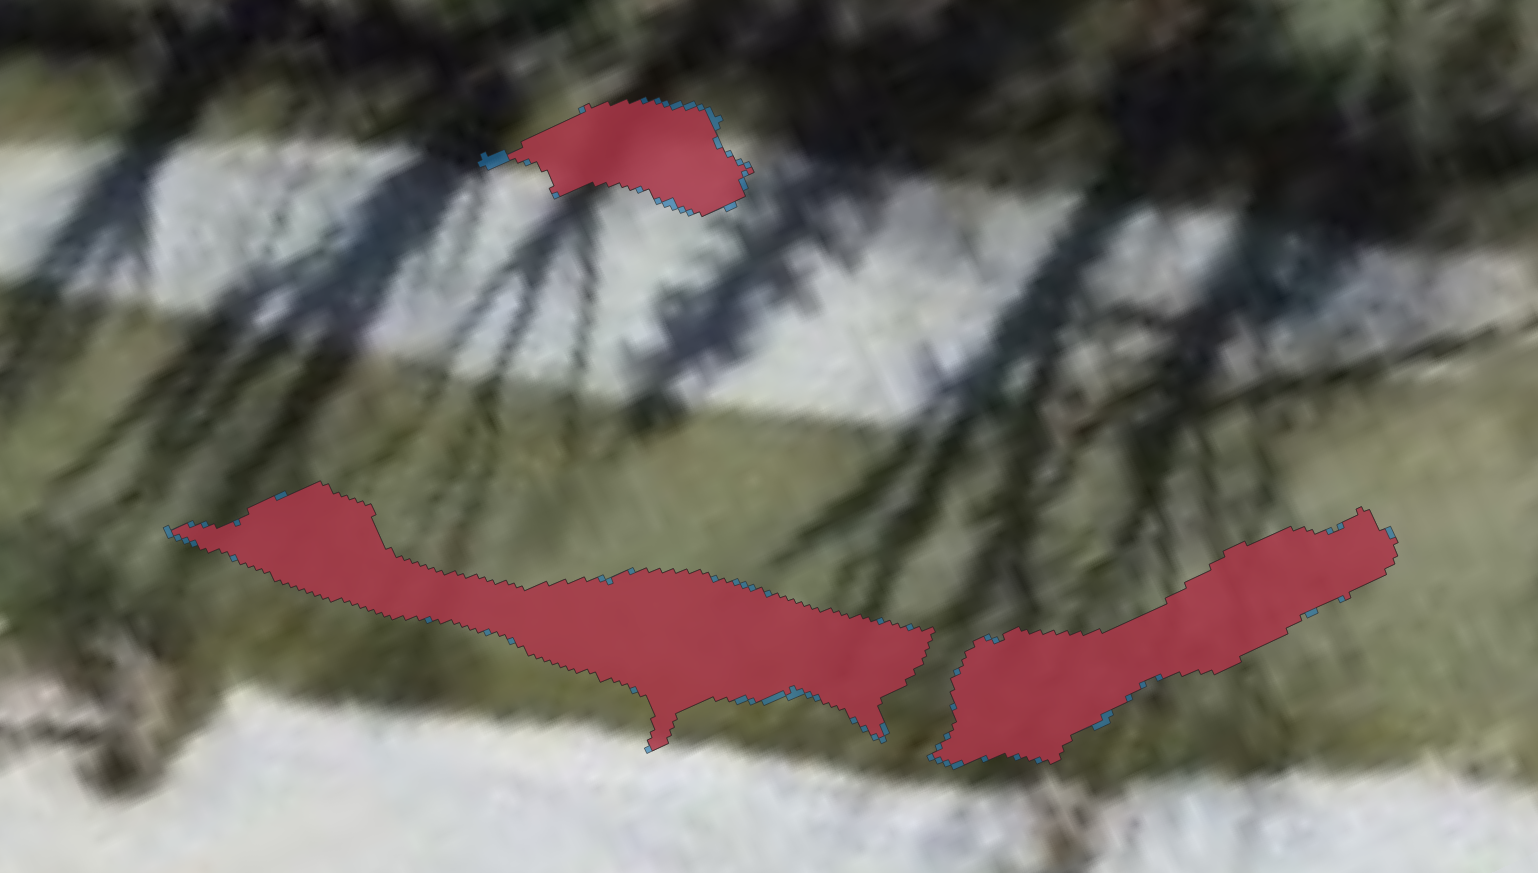
\includegraphics[width=\textwidth]{Bilder/param_combi_3_general_agreement.png}
	\caption{CWPs generated during trial run 3. Polygons of the speed-optimized algorithm are shown in red, and polygons of the original algorithm are shown in blue. The two algorithms are in general agreement, but do not fully agree at the pixel level.}
	\label{fig:param_combi_3_general_agreement}
\end{figure}

Figure \ref{fig:trial_run_1_more_pronounced_dis} shows an example of more pronounced disagreement between the two functions for trial run 1, figure \ref{fig:trial_run_perfect_agreement} shows an example set of cwps with perfect agreement between the two methods

\begin{figure}[H]
	\centering
	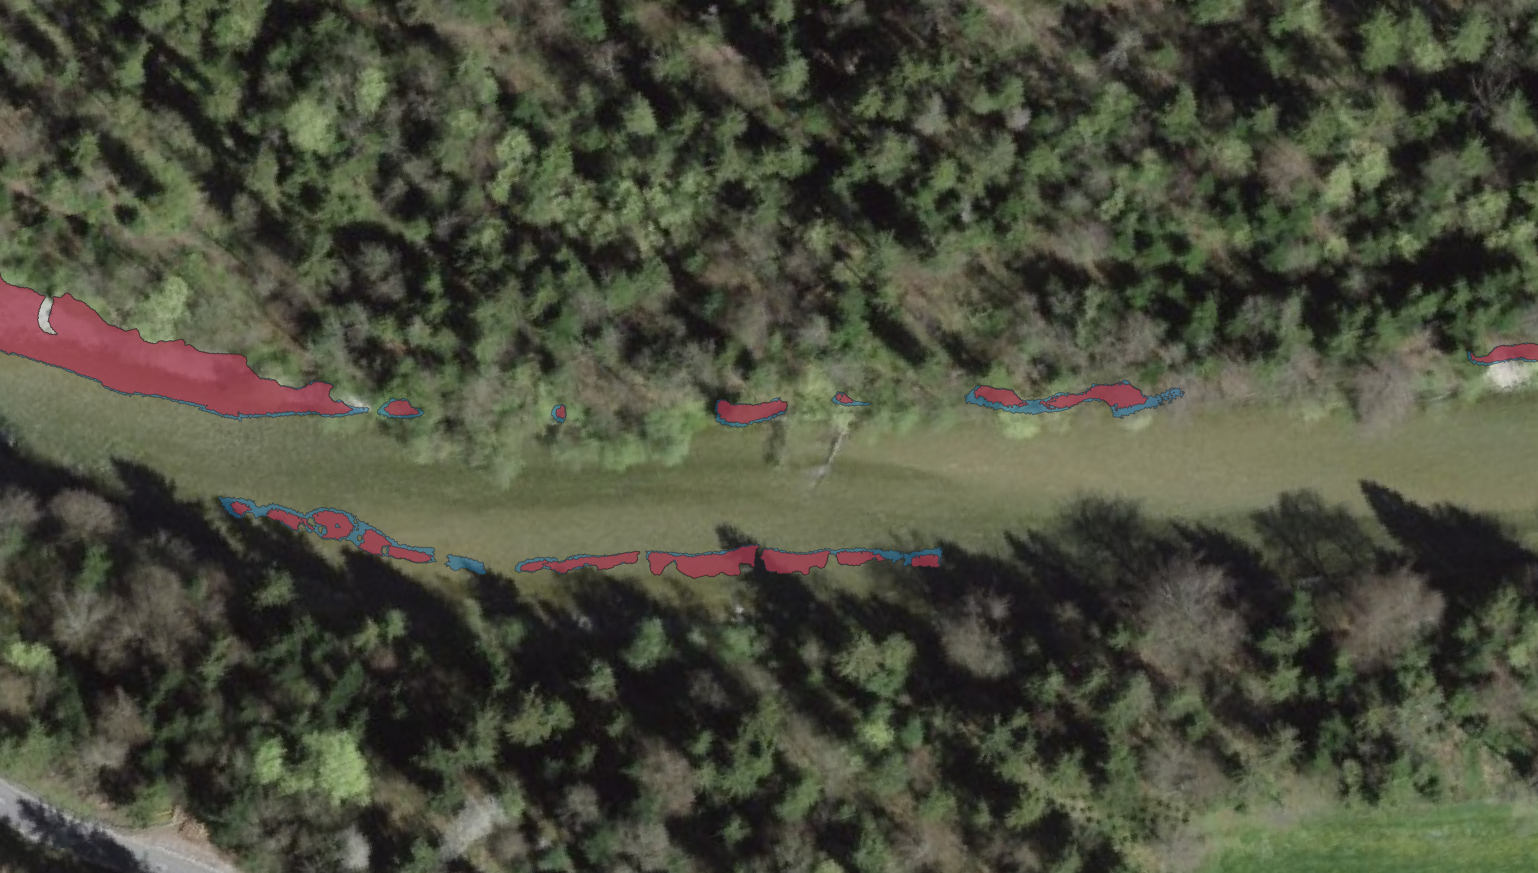
\includegraphics[width=\textwidth]{Bilder/trial_run_1_more_pronounced_dis.png}
	\caption{TODO}
	\label{fig:trial_run_1_more_pronounced_dis}
\end{figure}

\begin{figure}[H]
	\centering
	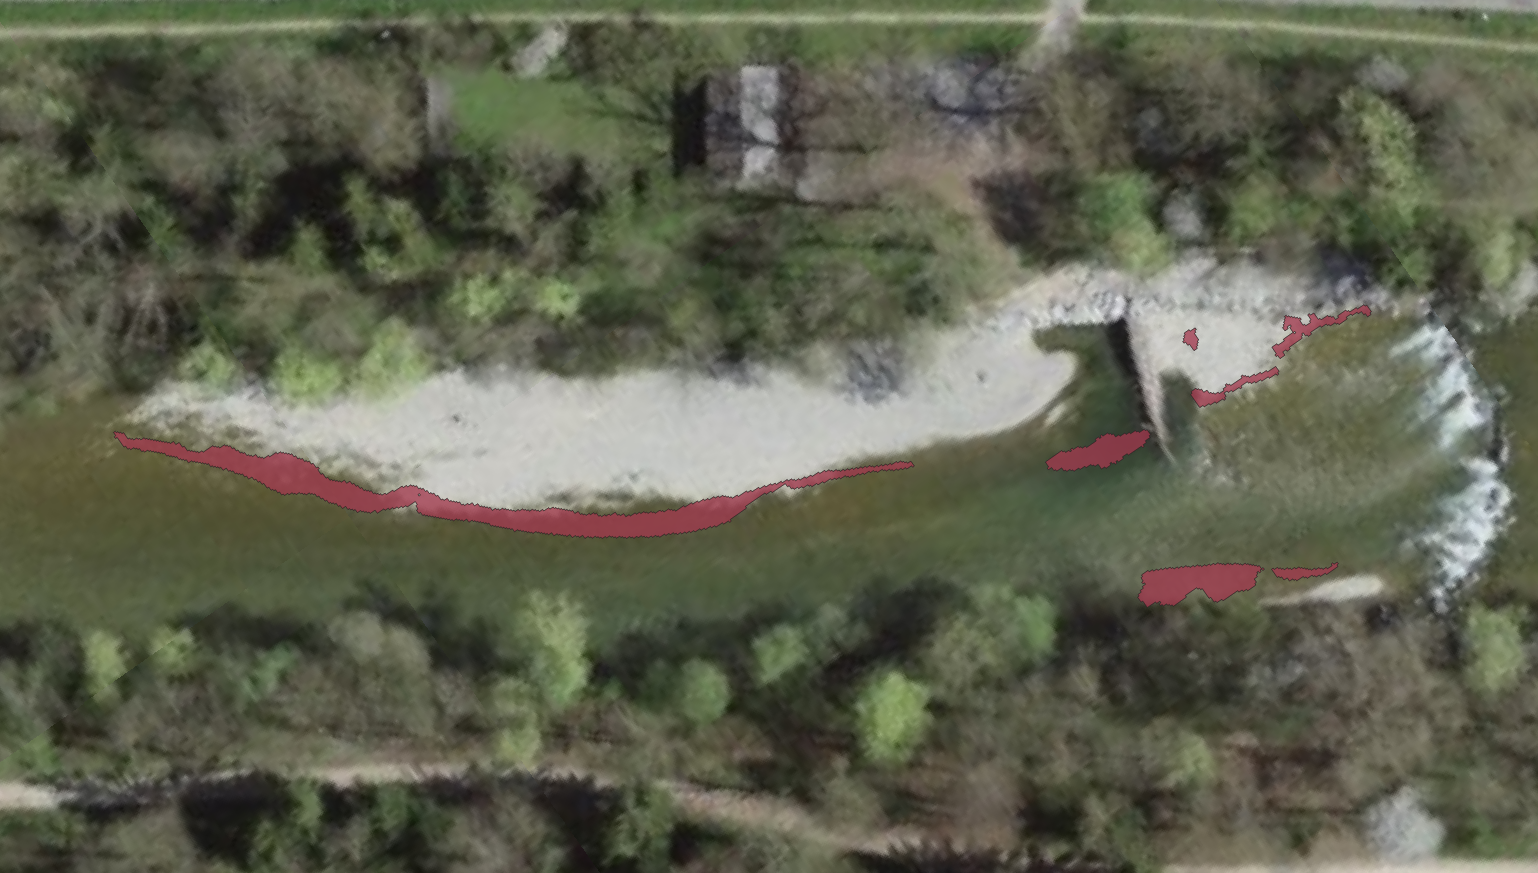
\includegraphics[width=\textwidth]{Bilder/trial_run_perfect_agreement.png}
	\caption{TODO}
	\label{fig:trial_run_perfect_agreement}
\end{figure}





\section{Speed comparison in execution}

% a simple line plot showing two lines with different collor. On the x-axis the step length, on the y axis execution time. One line is the execution speed of the optimized algorithm, the other line is the execution speed of the non optimized algorithm.

% It should be visible that the execution time of the new algorithm is shorter and generally constant over the step length parameter. The older version is slower and scales to longer execution speeds for smaller step lengths.

Figure \ref{fig:speed_comparison} shows the execution speed of the original aswell as the speed optimized cwp function. On the y-axis the execution speed in hours is ploted, on the x-axis the step-length parameter is ploted in meters. Execution speed is a constant half hour for teh speed optimized version where the original function ranges between 2 and 1.25 hours for the three runs whith hihger exeuction times for shorter step lengths.


\begin{figure}[ht]
	\centering
	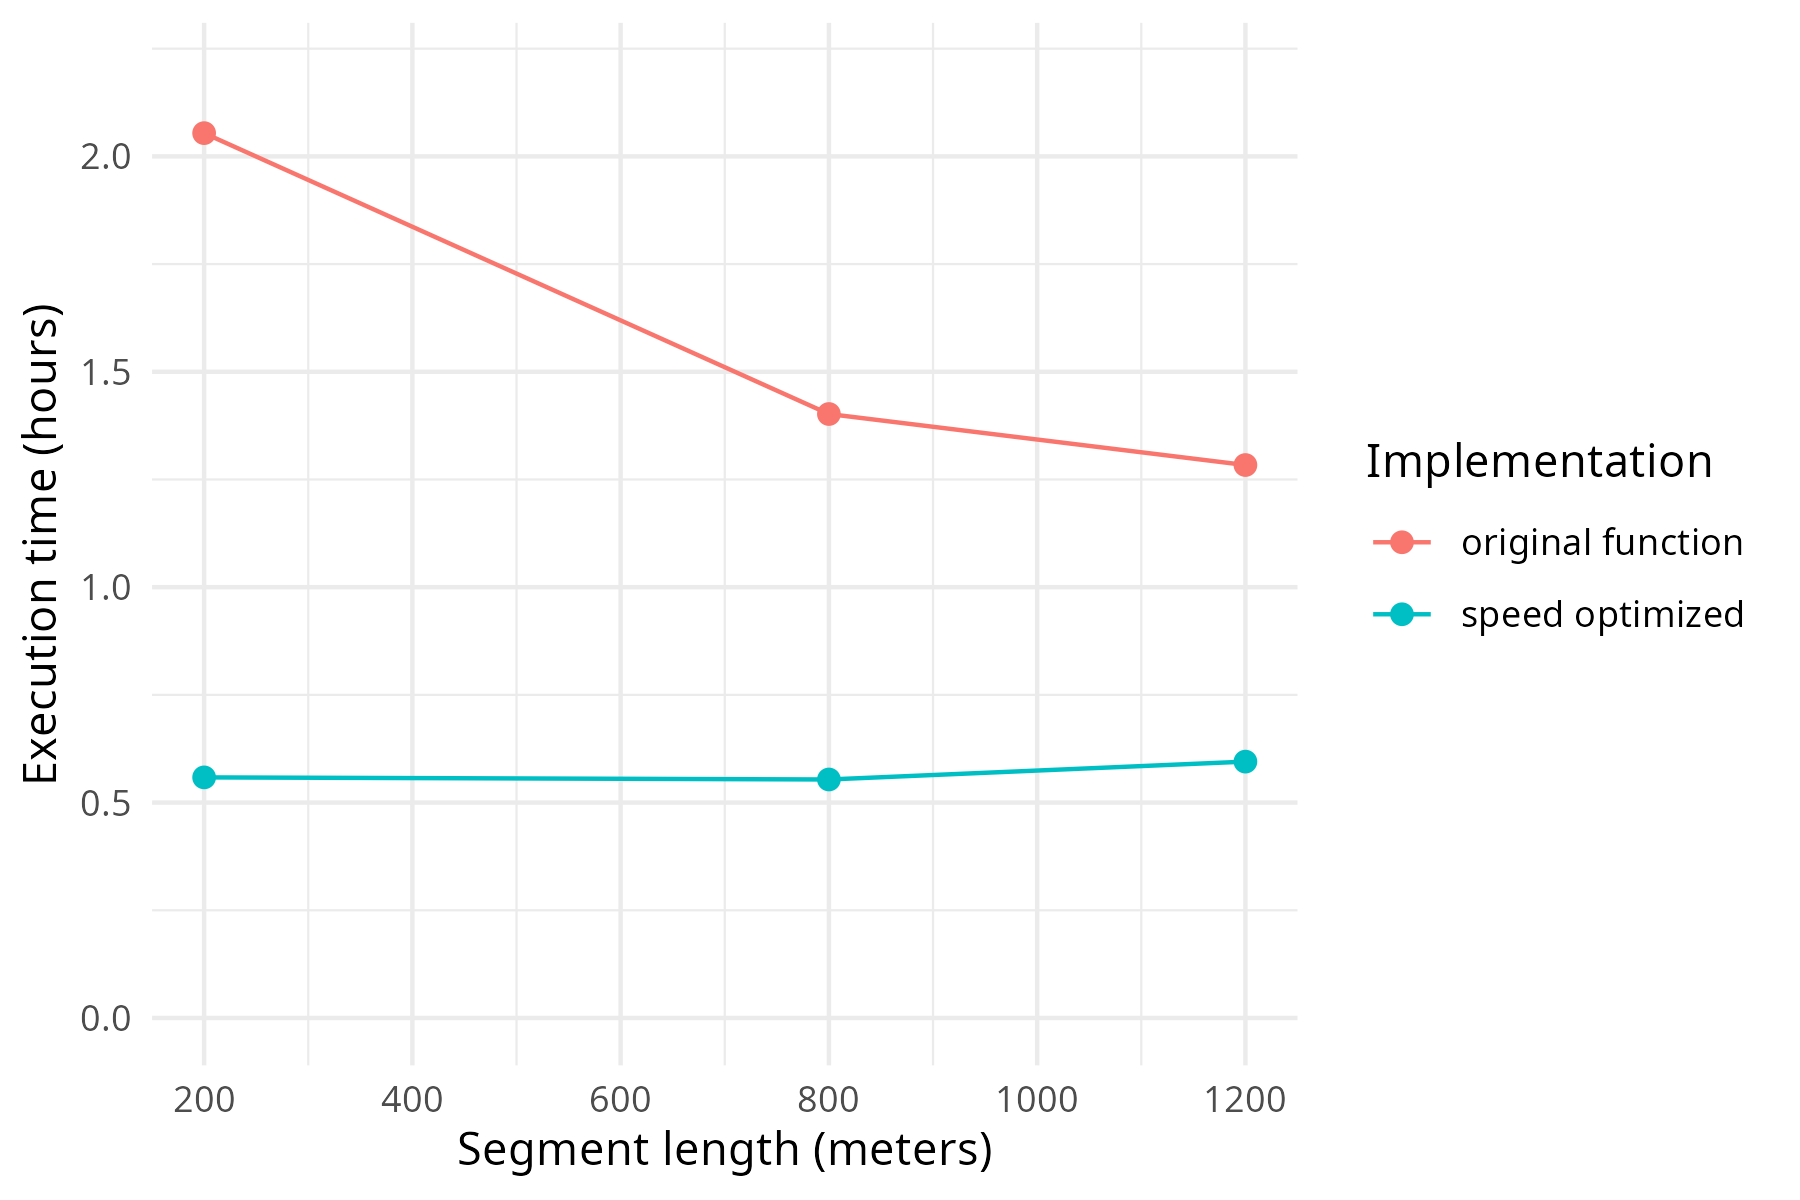
\includegraphics[width=0.8\textwidth]{Bilder/speed_comparison.png}
	\caption{Execution time of the original (v1) and optimized (v2) implementations of \texttt{detect\_cwp\_single} as a function of segment length. The optimized implementation shows execution times that are both shorter and largely constant across segment lengths, whereas the original implementation scales disproportionately with decreasing segment length (i.e., increasing number of segments).}
	\label{fig:speed_comparison}
\end{figure}




\section{Sensitiviy scores for step length parameter}

% include a plot of mu star and sigma for the non tributary caused and the tributary caused cold water patches. Also briefly introduce what is visible on the plot. 

% the plot shows boxplots of the mu.star and sigma sensitivity parameters for the xyz classified cold water patches. Red shows the tributary caused, blue the non tributary caused cold water patches. On the


Figure \ref{fig:step_length_sensitivity} shows morris sensitivity indices sigma and mustar with regards to the step length parameter. It can be seen that all non tributary caues CWP have a sensitivity index below 0.2. The spread in mu star for the sensitivity caused cwp is larger with some cwp featuring a similar sensitivity as the non tributary caused cwp and some featuing a substantially larger sensitivity value ( 0.3 and 0.6). The mean of both mu.star boxplots are very similar for both classes. 

\begin{figure}[ht]
	\centering
	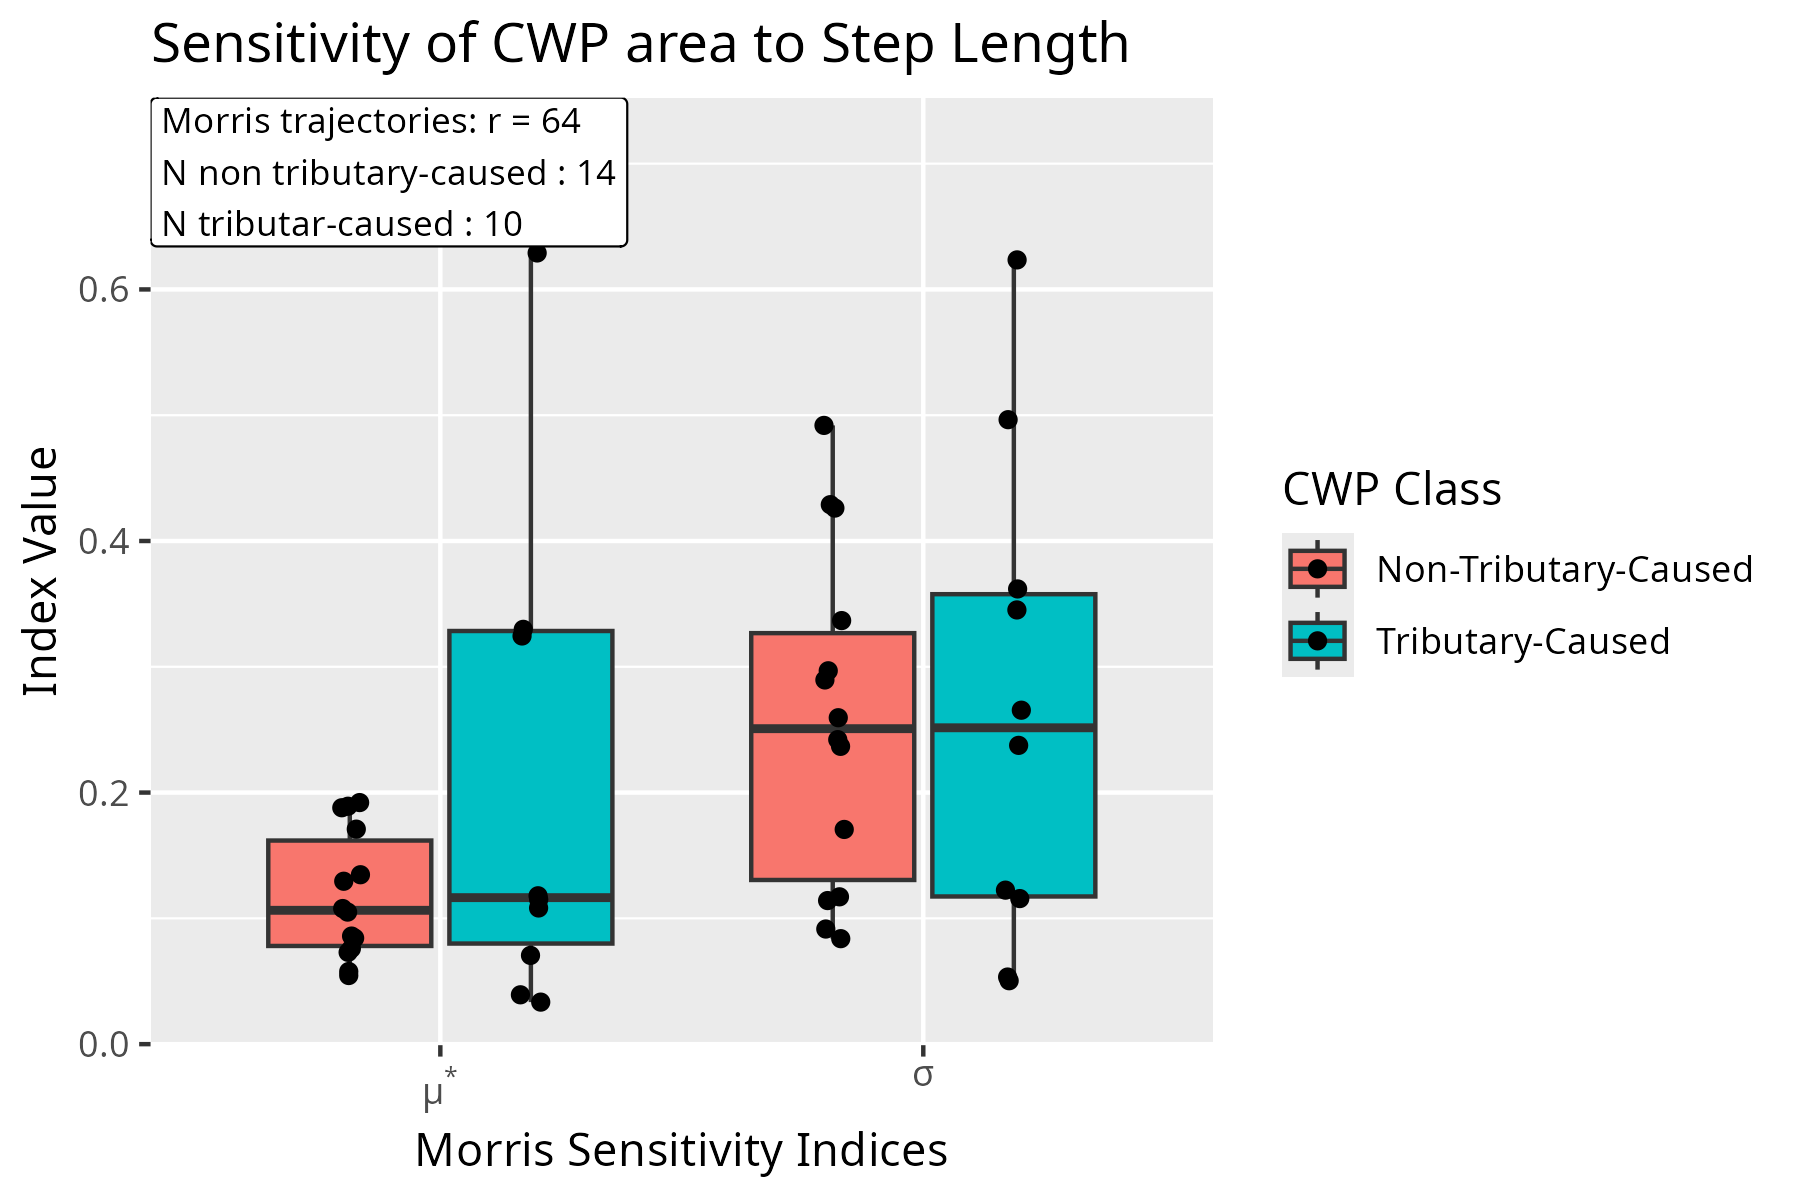
\includegraphics[width=0.8\textwidth]{Bilder/step_length_results.png}
	\caption{Morris sensitivity indices ($\mu^*$ and $\sigma$) for the \texttt{step\_length} parameter with respect to cold water patch area, stratified by patch class (red: tributary-caused; blue: non-tributary-caused). Boxplots show the distribution across bounding boxes, with sample sizes ($n$) given below each box.}
	\label{fig:step_length_sensitivity}
\end{figure}

\newpage

\section{Mu star for all parameters over all CWP}

% inlclude a plot of mu star for buffer bixels delta_T and also the step length for all cwp. Describe what the plot shows.

% the plot shows boxplots if mu star for the three different parameters buffer px, delta_T and also step length for all classified cwp. Each boxplot shows the distribution of the different mu.star values per location/area.


% further subsections are needed here for shure. Because in the discussion for instance i am also going to address the fact, that i think only the large tributary cwp are realy affected by this issue.

Figure \ref{fig:mu_star_overall} displays the mu.star values of all cwp with respect to the three different parameters varied during the morris experiment. The buffer pixel count continuously scores very low mu.star values while the step length and the temperature delta deviate from zero. Especially the temperature delta seems to highly influence the cwp with respect to their area.

\begin{figure}[ht]
	\centering
	
\includegraphics[width=0.8\textwidth]{Bilder/mu_star_res.png}
	\caption{Overall $\mu^*$ sensitivity indices for \texttt{buffer\_px}, \texttt{delta\_T}, and \texttt{step\_length} across all classified cold water patches ($N = 24$ locations, $r = 64$ trajectories).}
	\label{fig:mu_star_overall}
\end{figure}


\section{Mu.star and size for every cwp}

% include a plot showing mu.star in one axis and on the other axis the size of the cwp. Color the dots after the group membership. The large tributary caused patches should also have a large mu.star where smaller tributary caused patches might have a smaller mu star.


Figure  \ref{fig:mu_star_vs_area} shows the 24 selected cpw along 3 different dimensions. On the x axis, the averaged cwp area over all morris runs is depicted, on the y axis the sensitivty against the step length parameter is depicted. The color is used to indicate the average temperature delta to the surrounding environment averaged over all morris runs is depicted. The shape is indicating the class of the cwp.

\begin{figure}[ht]
	\centering
	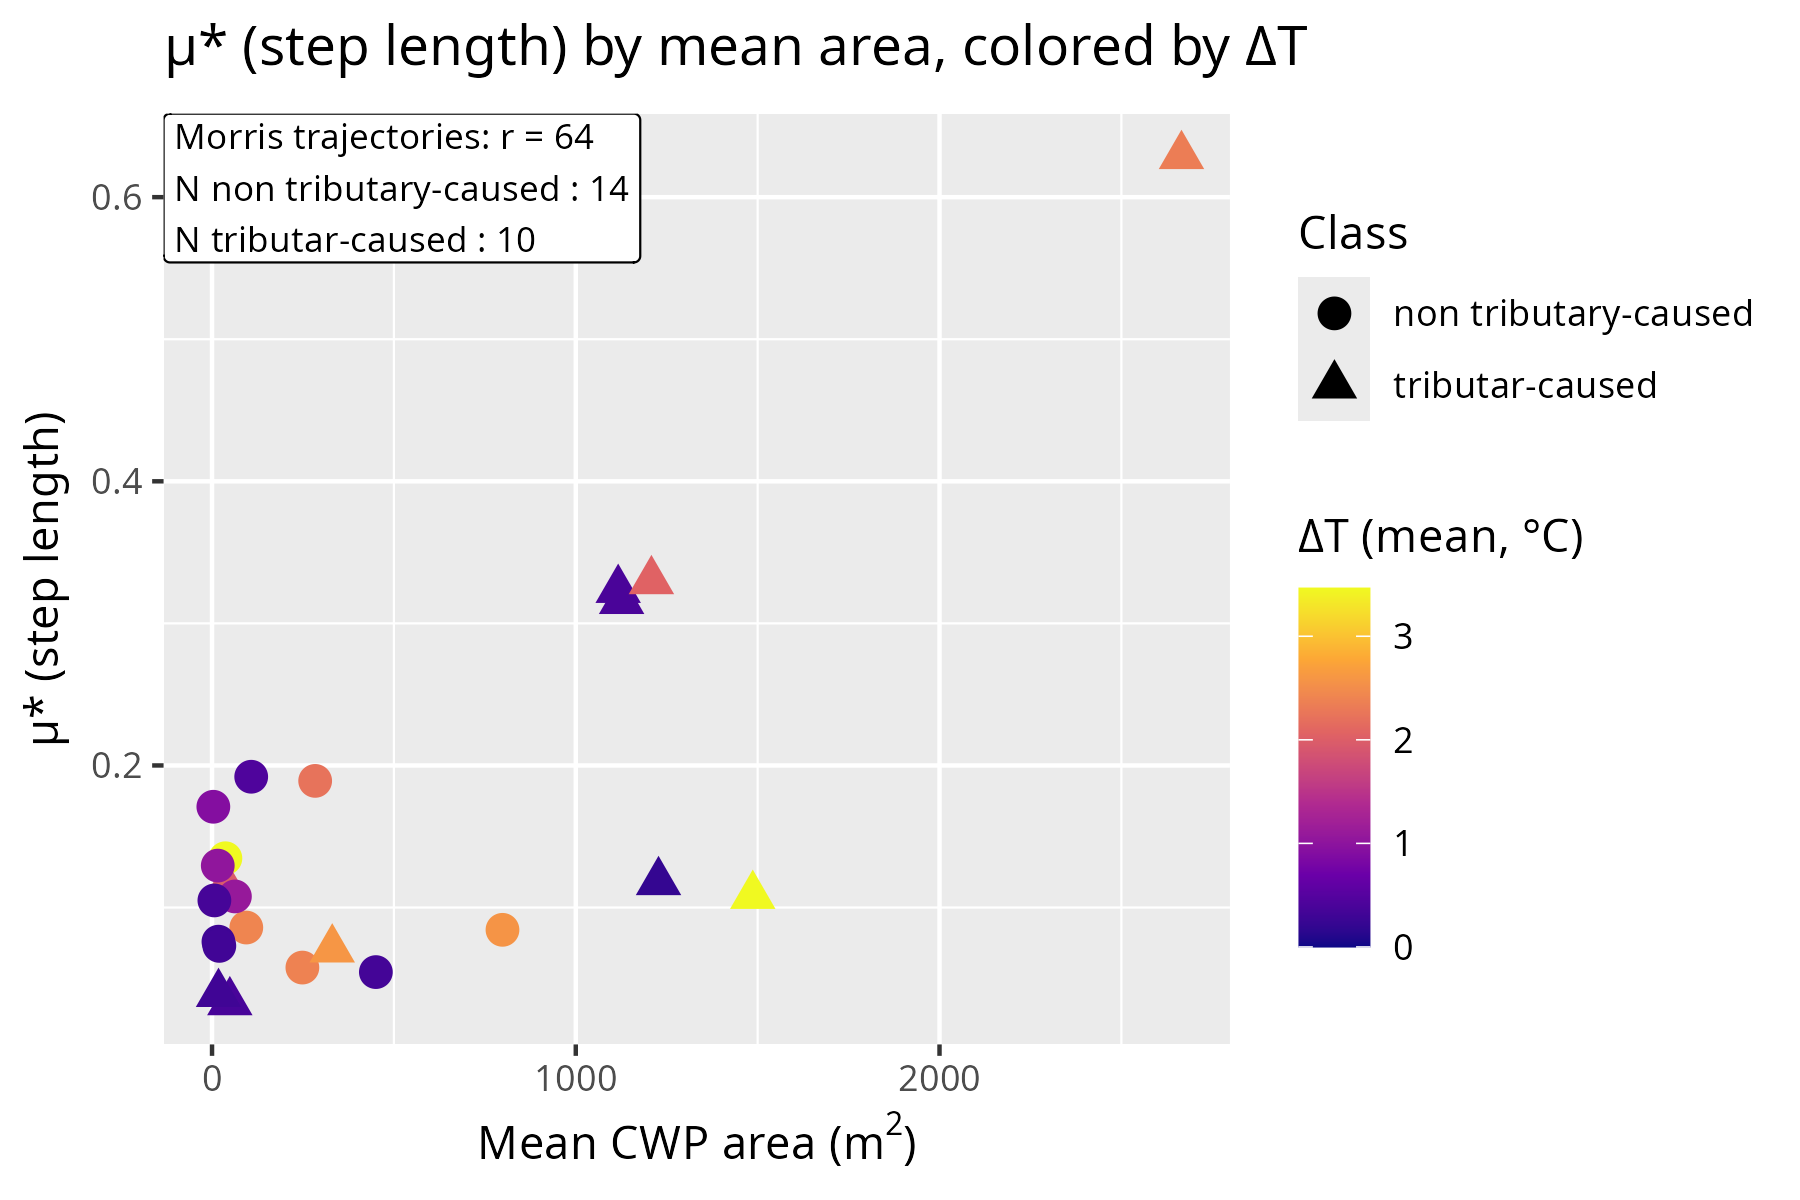
\includegraphics[width=0.8\textwidth]{Bilder/mu_star_vs_area_vs_deltaT.png}
	\caption{$\mu^*$ (step length) versus mean CWP area for each annotated location, colored by patch class.}
	\label{fig:mu_star_vs_area}
\end{figure}


\begin{table}[h]
	\centering
	\caption{Regression results for $\mu^*$ predicted by mean area and mean $\Delta T$}
	\label{tab:regression_mustar}
	\begin{tabular}{lrrrr}
		\toprule
		Predictor & Estimate & SE & $t$ & $p$ \\
		\midrule
		(Intercept)        & $9.024 \times 10^{-2}$  & $3.094 \times 10^{-2}$ & 2.92  & 0.009 \\
		Mean area          & $1.578 \times 10^{-4}$  & $2.839 \times 10^{-5}$ & 5.56  & $<0.001$ \\
		Mean $\Delta T$    & $-1.041 \times 10^{-2}$ & $1.739 \times 10^{-2}$ & $-0.60$ & 0.556 \\
		\bottomrule
	\end{tabular}
	
	\vspace{0.5em}
	\footnotesize
	\textit{Note.} $R^2 = 0.611$, Adjusted $R^2 = 0.572$, $F(2, 20) = 15.73$, $p < 0.001$. Residual standard error $= 0.088$ on 20 degrees of freedom (one observation deleted due to missingness).
\end{table}
